\documentclass[11pt]{article}

% Change "review" to "final" to generate the final (sometimes called camera-ready) version.
% Change to "preprint" to generate a non-anonymous version with page numbers.
\usepackage[preprint]{acl}

\usepackage{times}
\usepackage{latexsym}

\usepackage[T1]{fontenc}

\usepackage[utf8]{inputenc}
\usepackage{microtype}
\usepackage{inconsolata}
\usepackage{graphicx}
\usepackage{subcaption}

\usepackage{tikz}
\usetikzlibrary{positioning, fit, backgrounds, arrows.meta}

\title{Adaptive MoEUT}

\author{Marta Muskus\\
  University of Warsaw \\
  \texttt{m.muskus@student.uw.edu.pl} \\\And
  Adrian Boguszewski  \\
  University of Warsaw \\
  \texttt{a.boguszews2@student.uw.edu.pl}
}

\begin{document}
\maketitle
\begin{abstract}
    TODO
\end{abstract}

\section{Introduction}
\textit{Universal Transformers} (UTs) are not a new idea \cite{ut}.
They are a variation of the \textit{Vanilla Transformer} (VT) \cite{transformer} architecture that achieves network depth not via stacking multiple transformer blocks, but rather reusing the same blocks in a loop.
They are the spiritual ancestor of \textit{Recurrent Neural Networks} (RNNs) in the transformer paradigm and are usually designed either as pure cycles or cycles with additional initial and final layers (see Figure~\ref{fig:ut-designs}).

Proponents of this architecture argue that they generalize better - that the built-in recursion allows the models to decompose structured problems, and generalize to longer sequences \cite{moeut}.
However the weight-sharing also introduces some scaling-related problems, because a UT that loops $N$ times is equivalent in depth to a $N$ layer VT, but only has $\frac{1}{N}$ parameters.
One of the ideas to combat this issue is to make the UT's layer $N$ times wider, which would result in a usually prohibitive jump in compute and memory requirements.
Another approach is to modify the UT's architecture to introduce some sparsity like in \textit{Mixture-of-Experts} (MoE) \cite{moe}.
This results in a larger parameter count that is arbitrarily scalable, while fixing the compute and memory requirements.

\textit{Mixture-of-Experts Universal Transformer} (MoEUT) \cite{moeut} is a UT architecture that injects sparsity to both the attention computation via \textit{SwitchHead} \cite{switchhead}, and the feedforward layer via $\sigma$-MoE.

In this work we attempt to extend the MoEUT design with \textit{Adaptive Compute Time} (ACT) by using the Stick-breaking Halting algorithm proposed in the \textit{Sparse Universal Transformer} \cite{sut}.

\begin{figure}[htbp]
    \centering
    \begin{subfigure}[a]{0.45\textwidth}
        \centering
        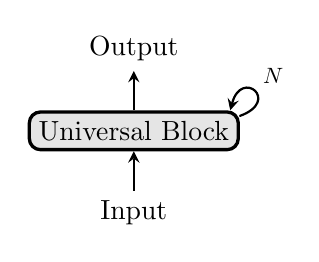
\begin{tikzpicture}[
            module/.style={draw, very thick, rounded corners, minimum width=15ex},
            ubmodule/.style={module, fill=gray!20},
            arrow/.style={-stealth, thick}, 
            corner loop/.style={-stealth, thick, line cap=round}
        ]
            \node (in) {Input};
            \node [above=0.5cm of in, ubmodule, align=center] (ub) {Universal Block};
            \node [above=0.5cm of ub] (out) {Output};

            \draw [arrow] (in) -- (ub);
            \draw [arrow] (ub) -- (out);
            
            \draw [corner loop] (ub.8) to [out=20, in=75, looseness=10] node[above right, midway, scale=0.8] {$N$} (ub.12);

        \end{tikzpicture}
        \caption{Cycle}
    \label{cycle}
    \end{subfigure}
    \hfill
    \begin{subfigure}[b]{0.45\textwidth}
        \centering
        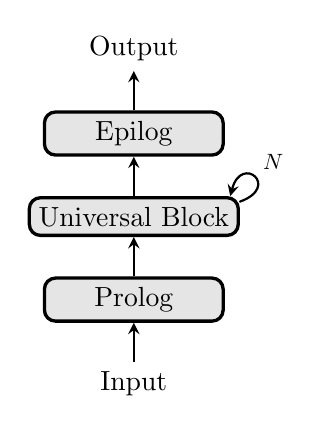
\begin{tikzpicture}[
            module/.style={draw, very thick, rounded corners, minimum width=15ex},
            pmodule/.style={module, fill=gray!20},
            emodule/.style={module, fill=gray!20},
            ubmodule/.style={module, fill=gray!20},
            arrow/.style={-stealth, thick}, 
            corner loop/.style={-stealth, thick, line cap=round}
        ]
            \node (in) {Input};
            \node [above=0.5cm of in, pmodule, align=center] (p) {Prolog};
            \node [above=0.5cm of p, ubmodule, align=center] (ub) {Universal Block};
            \node [above=0.5cm of ub, emodule, align=center] (e) {Epilog};
            \node [above=0.5cm of e] (out) {Output};

            \draw [arrow] (in) -- (p);
            \draw [arrow] (p) -- (ub);
            \draw [arrow] (ub) -- (e);
            \draw [arrow] (e) -- (out);
            
            \draw [corner loop] (ub.8) to [out=20, in=75, looseness=10] node[above right, midway, scale=0.8] {$N$} (ub.12);

        \end{tikzpicture}
        \caption{Middle Cycle}
        \label{middle-cycle}
    \end{subfigure}
    \caption{UT Architectures}
    \label{fig:ut-designs}
\end{figure}

\section{Model Architecture}

\subsection{Overview}
TODO

\subsection{Transformer Block}
TODO

\begin{figure}
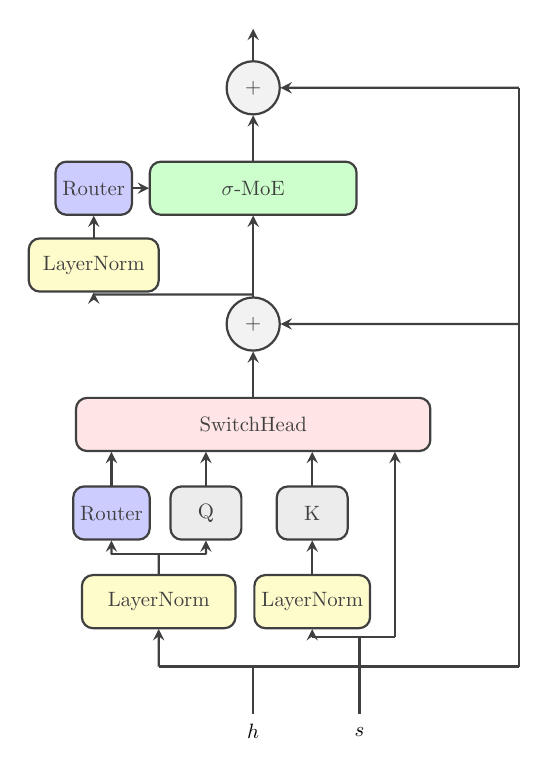
\begin{tikzpicture}[
    module/.style={draw, thick, darkgray, minimum height=0.9cm, align=center, rounded corners},
    lnorm/.style={module, fill=yellow!20},
    sel/.style={module, fill=blue!20, minimum width=1.2cm},
    proj/.style={module, fill=gray!15, minimum width=1.2cm},
    att/.style={module, fill=pink!40},
    moe/.style={module, fill=green!20},
    plus/.style={draw, thick, darkgray, circle, fill=gray!10, minimum size=0.9cm, inner sep=0pt},
    arrow/.style={-stealth, thick, darkgray},
    line/.style={thick, darkgray},
    rounded corners=1pt,
    scale=0.75, transform shape
]
    \begin{scope}[local bounding box=input_layer]
        \node (h_in) at (0, -0.7) {$h$};
        \node (s_in) at (1.8, -0.7) {$s$};
    \end{scope}

    \begin{scope}[local bounding box=bottom_block]
        
        % --- h Stream ---
        \draw[line] (0, -0.4) -- (0, 0.4);
        
        % Split h: Left to Layernorm, Right to main Residual Spine
        \draw[line] (0, 0.4) -- (-1.6, 0.4);
        \node[lnorm, minimum width=2.6cm] (lnorm_h) at (-1.6, 1.5) {LayerNorm};
        \draw[arrow] (-1.6, 0.4) -- (lnorm_h.south);
        
        % Projections from Layernorm_h
        \node[sel] (sel_h) at (-2.4, 3.0) {Router};
        \node[proj] (q) at (-0.8, 3.0) {Q};
        
        \draw[line] (lnorm_h.north) -- (-1.6, 2.3);
        \draw[line] (-1.6, 2.3) -- (-2.4, 2.3); 
        \draw[arrow] (-2.4, 2.3) -- (sel_h.south);
        \draw[line] (-1.6, 2.3) -- (-0.8, 2.3); 
        \draw[arrow] (-0.8, 2.3) -- (q.south);
        
        % --- s Stream ---
        % Using preaction to smoothly jump over the h residual line
        \draw[line, preaction={draw, white, line width=4pt}] (1.8, -0.4) -- (1.8, 0.9);
        
        % Split s: Left to Layernorm (for K), Right straight up (for V)
        \draw[line] (1.8, 0.9) -- (1.0, 0.9);
        \node[lnorm, minimum width=1.4cm] (lnorm_s) at (1.0, 1.5) {LayerNorm};
        \draw[arrow] (1.0, 0.9) -- (lnorm_s.south);
        
        % Projection from Layernorm_s
        \node[proj] (k) at (1.0, 3.0) {K};
        \draw[arrow] (lnorm_s.north) -- (k.south);
        
        % The unprojected 's' routing for attention value
        \draw[line] (1.8, 0.9) -- (2.4, 0.9);
    \end{scope}

    % ==========================================
    % LAYER 2: Attention Block
    % ==========================================
    \begin{scope}[local bounding box=mid_block]
        % SwitchHead sized to perfectly bracket the outer inputs (sel_h and s_val)
        \node[att, minimum width=6.0cm] (switchhead) at (0, 4.5) {SwitchHead};
        
        % Arrows ascending into SwitchHead
        \draw[arrow] (sel_h.north) -- (sel_h.north |- switchhead.south);
        \draw[arrow] (q.north) -- (q.north |- switchhead.south);
        \draw[arrow] (k.north) -- (k.north |- switchhead.south);
        \draw[arrow] (2.4, 0.9) -- (2.4, 0.9 |- switchhead.south); % Raw s (Value)
    \end{scope}

    % ==========================================
    % LAYER 3: Residual & MoE Block (h stream only)
    % ==========================================
    \begin{scope}[local bounding box=top_block]
        % First Residual Addition
        \node[plus] (plus1) at (0, 6.2) {$+$};
        \draw[arrow] (switchhead.north) -- (plus1.south);
        
        % Establish the main right-side Residual line for h
        \draw[line] (0, 0.4) -- (4.5, 0.4);
        \draw[line] (4.5, 0.4) -- (4.5, 6.2);
        \draw[arrow] (4.5, 6.2) -- (plus1.east);
        
        % MoE Nodes
        \node[moe, minimum width=3.5cm] (moe) at (0, 8.5) {$\sigma$-MoE};
        \node[lnorm, minimum width=2.2cm] (lnorm_moe) at (-2.7, 7.2) {LayerNorm};
        \node[sel] (sel_moe) at (-2.7, 8.5) {Router};
        
        % MoE Routing (From + to Layernorm/MoE)
        \coordinate (moe_split) at (0, 6.7);
        \draw[line] (plus1.north) -- (moe_split);
        \draw[arrow] (moe_split) -- (moe.south);
        
        \draw[line] (moe_split) -- (-2.7, 6.7);
        \draw[arrow] (-2.7, 6.7) -- (lnorm_moe.south);
        \draw[arrow] (lnorm_moe.north) -- (sel_moe.south);
        \draw[arrow] (sel_moe.east) -- (moe.west);
        
        % Second Residual Addition
        \node[plus] (plus2) at (0, 10.2) {$+$};
        \draw[arrow] (moe.north) -- (plus2.south);
        
        % Continue main residual spine up to top +
        \draw[line] (4.5, 6.2) -- (4.5, 10.2);
        \draw[arrow] (4.5, 10.2) -- (plus2.east);
        
        % Final Output
        \draw[arrow] (plus2.north) -- (0, 11.2);
    \end{scope}

\end{tikzpicture}
\caption{Transformer Block}
\label{fig:transformer-block}
\end{figure}

\section{Experiments}

\subsection{Training}

\subsection{Evaluation}

\subsection{Adaptive Compute Time}

\section{Closing Remarks}

\section{Further Work}

% \section{Motivation and Context}

% Mixture-of-Experts Universal Transformer (MoEUT) \citep{moeut}  is an improvement of the Universal Transformer (UT) \citep{ut} architecture. The idea behind UT is to introduce extreme weight sharing into the traditional transformer by repeatedly processing tokens with a single transformer block instead of having multiple single-use blocks. MoEUT tries to improve the efficiency of a basic UT, by introducing Mixture-of-Experts in the feedforward networks \citep{moe} as well as the multihead attention mechanism \citep{switchhead}.


% We want to introduce Adaptive Compute Time (ACT) into the MoEUT architecture both at the token and loop level. MoEUT, as presented in the original paper, has a fixed number of loops where every loop processes every token. Every query gets the same amount of compute. The idea of ACT is that different queries require different amounts of compute e.g. we could get away with allocating less compute to easy queries and utilizing those savings for more difficult queries.


% In the case of UTs, ACT could mean adjusting the number of loops that the query goes through before producing an answer. This idea is explored in the LoopFormer and Sparse Universal Transformer \citep{sut} papers. This is what we refer to as loop level ACT. Another approach would be to adjust the amount of tokens that are processed in each loop. This idea is explored in the Mixture-of-Recursions \citep{mor} paper and we refer to it as token level ACT.


% As far as we know the two approaches were never combined - papers mentioned above either fixed the number of loops and adjusted the number of tokens processed (token-level ACT) or fixed the number of tokens processed and adjusted the number of loops (loop-level ACT). We would like to see if implementing both of them within a MoEUT would result in compute savings without sacrificing the  quality of the model.


% \section{Action Plan}

% \begin{enumerate}
%     \item Choose two model parameter sizes (e.g. 244M, 728M), training dataset and training compute budget.
%     \item Train baseline models - standard dense transformer, standard MoEUT.
%     \item Choose the evaluation dataset and metrics (e.g. loss, perplexity, accuracy and FLOPs or MACs spent on inference).
%     \item Evaluate baseline models.
%     \item Design the Fully Adaptive MoEUT architecture that combines token-level and loop-level ACT.
%     \item Train and evaluate the Fully Adaptive MoEUT model.
%     \item Compare the models and report findings.
% \end{enumerate}

% \section{Datasets and Benchmarks}

% As a training dataset we plan on using the Colossal Clean Crawled Corpus (C4), as it is one of the three datasets utilized in the original MoEUT paper. The quality of our Fully Adaptive MoEUT will be evaluated using several metrics. We plan on testing its zero-shot performance on the LAMBADA dataset and possibly further on HellaSwag and ARC. We will also measure cross-entropy loss and perplexity, as well as check if our model can match performance baselines while using fewer MACs/FLOPs.

\bibliography{references}        

\end{document}
